% ── 3. GRASP-RAG ─────────────────────────────────────────────────────────────
\section{GRASP-RAG}

\subsection{Dataset and Setup}

We evaluate on four domains from UltraDomain~\cite{ding2024ultradomain}:
Agriculture (17,272 entity nodes; 15,460 edges), CS (16,053; 14,173), Legal
(14,494; 20,423), and Health (32,428; 29,486).
For each domain, a single knowledge graph is constructed once using LightRAG's
pipeline---documents split into 1,200-token overlapping chunks, entity--relation
triples extracted by GPT-4o-mini~(\texttt{gpt-4o-mini-2024-07-18}) and
deduplicated, embeddings produced by \texttt{text-embedding-3-small}.
All methods (NaiveRAG, LightRAG, PathRAG, and GRASP-RAG) query this same graph,
so the sole experimental variable is the retrieval strategy.
NaiveRAG in this setup retrieves from KG-extracted content rather than raw
document chunks; its performance may therefore differ from NaiveRAG deployed
over unstructured text.

\subsection{Overview}

Figure~\ref{fig:system} shows the complete GRASP-RAG pipeline and multi-judge
evaluation protocol.
At query time: (1) a VDB search retrieves up to 20 candidate entity names from
the graph; (2) an LLM classifier infers the query type $\tau$ and anchor nodes
$\mathcal{A}$ from those candidates; (3) a motif-specific graph algorithm
retrieves the matching subgraph $\mathcal{S}$; (4) the context builder
linearizes $\mathcal{S}$ into a topology-aware text scaffold; and (5) an LLM
generates the answer from that scaffold.

% ── System Overview Figure (single-column) ───────────────────────────────────
\begin{figure}[t]
  \centering
  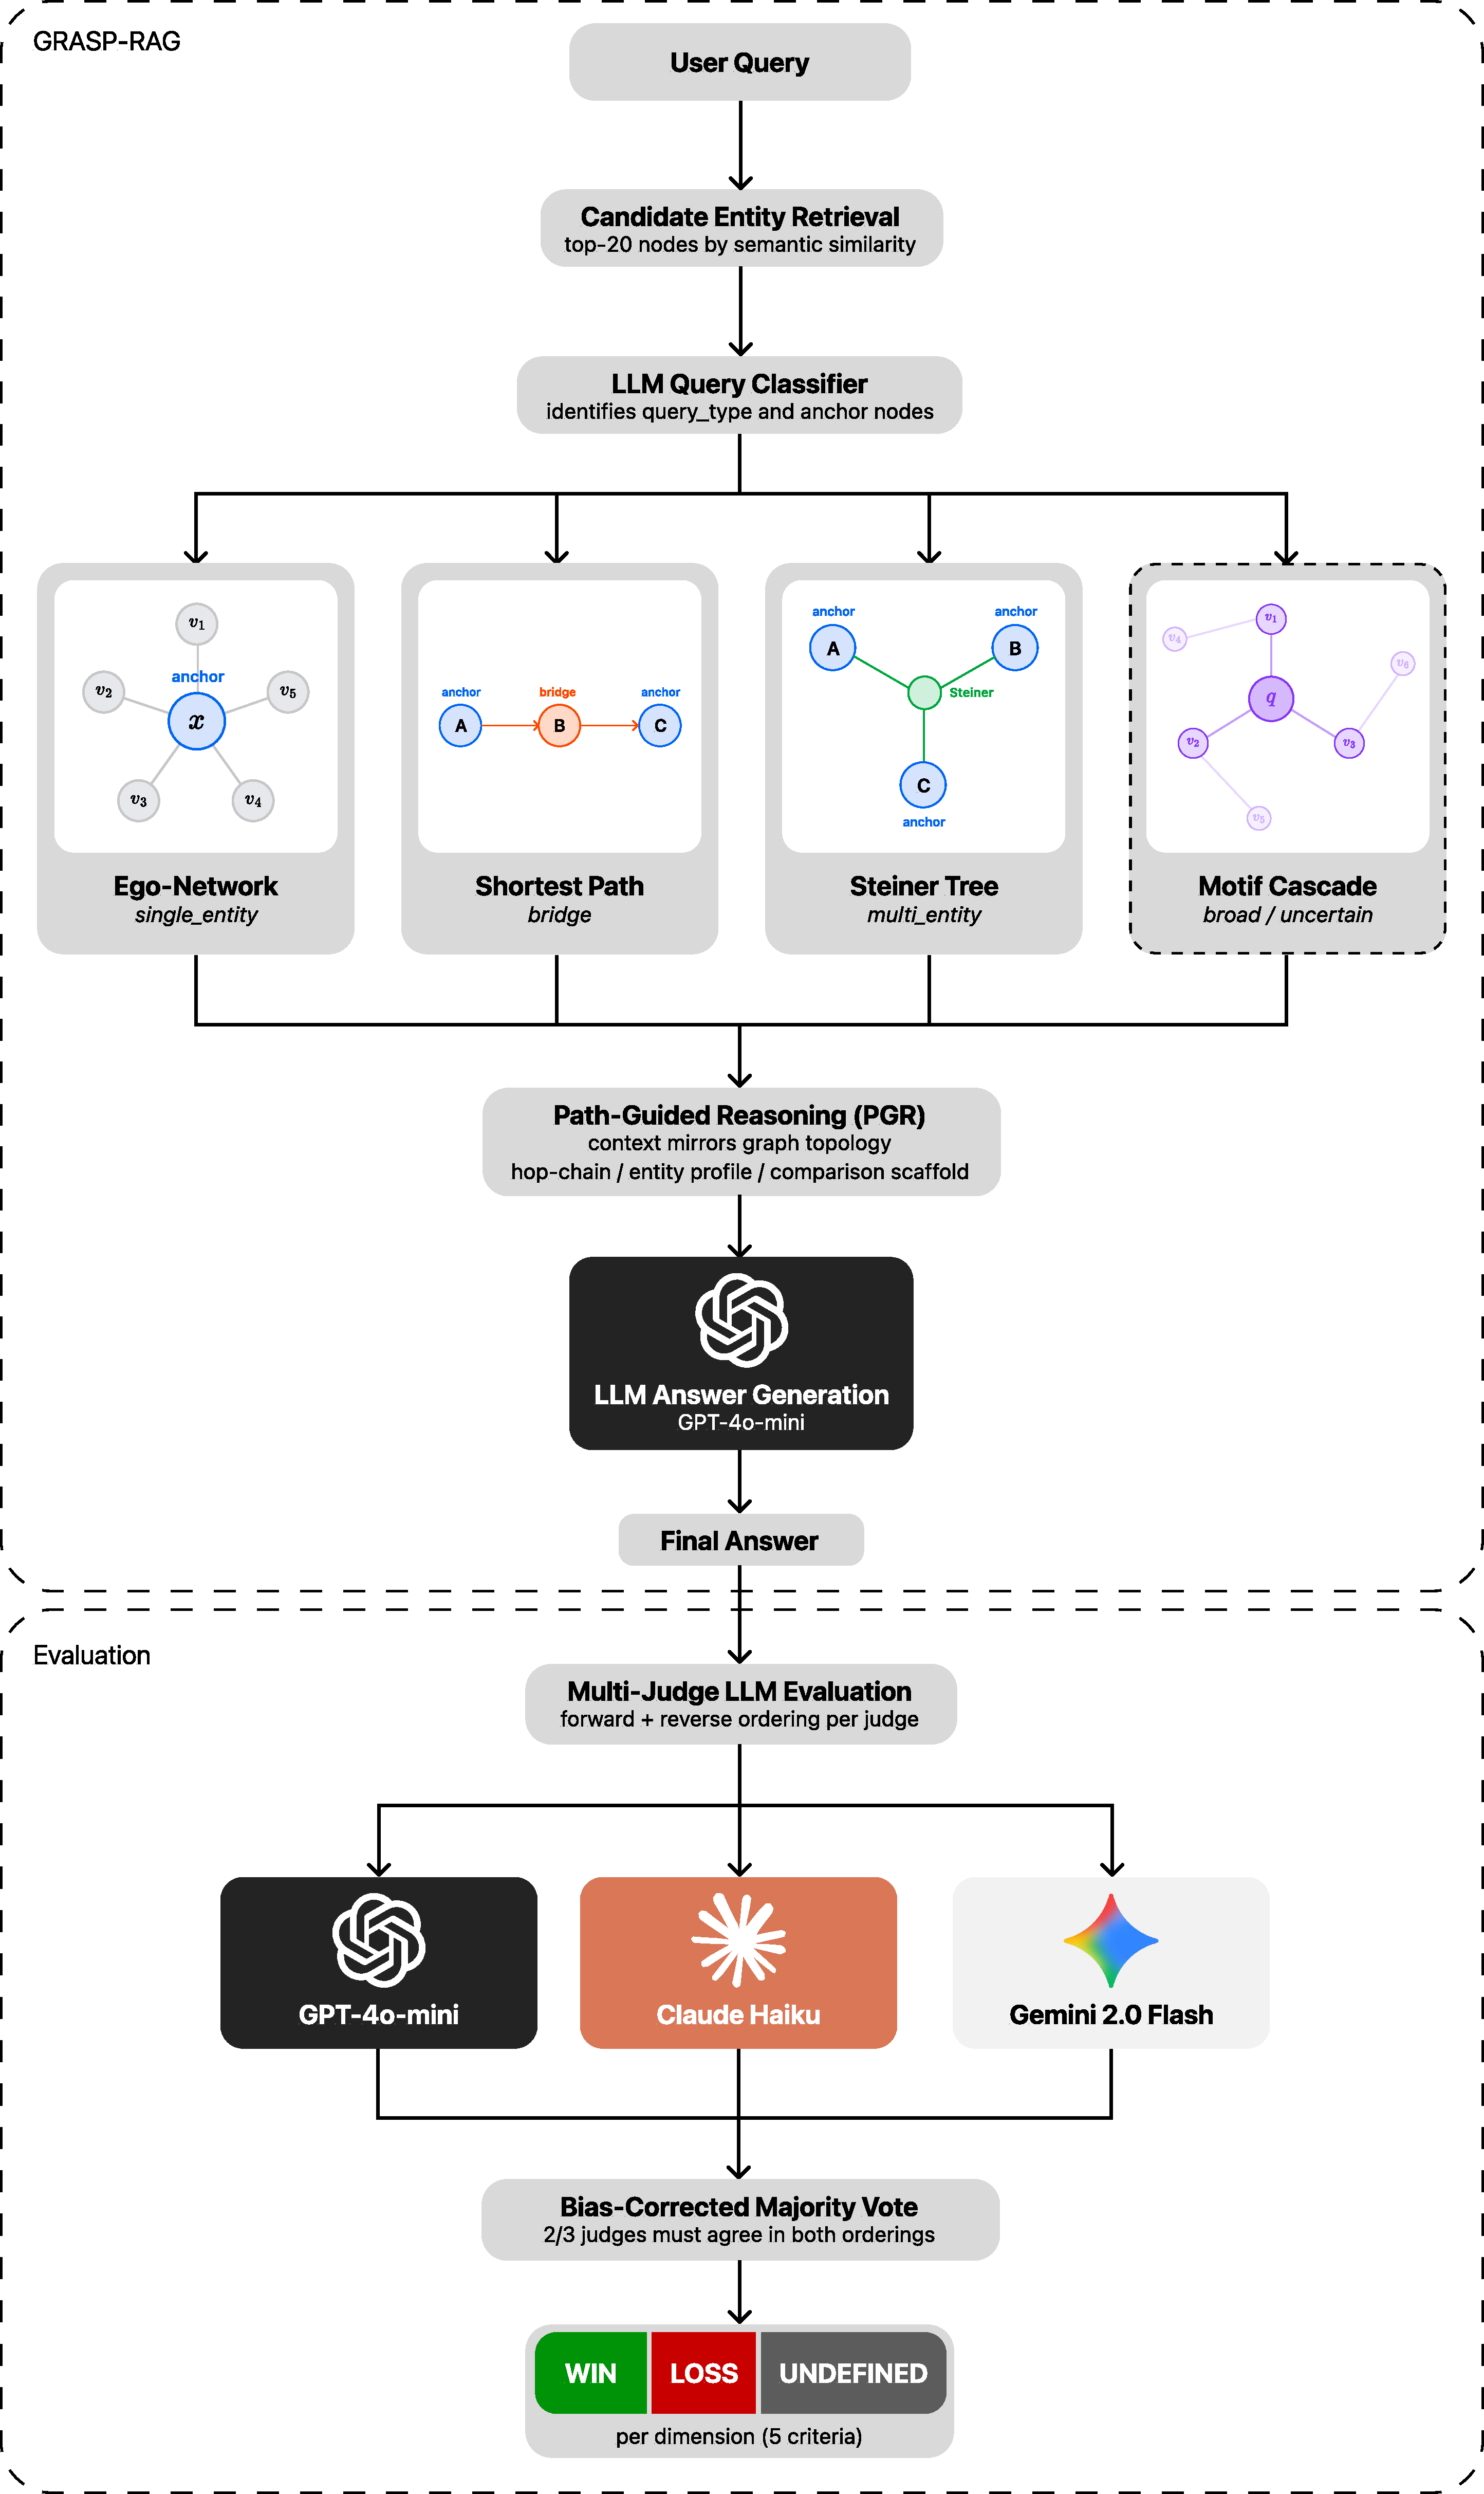
\includegraphics[width=\columnwidth]{system.pdf}
  \caption{GRASP-RAG system overview. \textbf{Top (pipeline):} a user query
    passes through candidate entity retrieval, an LLM classifier, one of four
    motif-specific graph algorithms (Ego-Network, Shortest Path, Steiner Tree,
    or hybrid fallback), and topology-aware context structuring before answer
    generation. \textbf{Bottom (evaluation):} three independent LLM judges
    (GPT-4o-mini, Claude Haiku, Gemini~2.0~Flash) each run forward and reversed
    orderings; a bias-corrected majority vote yields Win, Loss, or Undefined
    per dimension.}
  \label{fig:system}
\end{figure}

\subsection{Query Types and Retrieval Motifs}
\label{sec:motifs_table}

Table~\ref{tab:motifs} defines the four query types and their retrieval motifs,
and Figure~\ref{fig:motifs} illustrates the subgraph shape each one produces.
Each row maps a linguistic question shape to the graph algorithm whose subgraph
structure best matches the answer that shape requires.

\begin{table*}[t]
\caption{GRASP-RAG query types, retrieval motifs, prior-work inspiration, and
  example questions. The classifier routes each query to the matching motif at
  inference time. LightRAG hybrid also serves as the confidence-score fallback
  for any query type when $c(\mathcal{S}) < 0.04$; see
  \S\ref{sec:motif} (Confidence and fallback).}
\label{tab:motifs}
\centering
\renewcommand{\arraystretch}{1.25}
\setlength{\tabcolsep}{4pt}
\begin{tabular}{llp{2.6cm}p{3.6cm}p{5.0cm}}
\toprule
\textbf{Query Type} & \textbf{Motif} & \textbf{Algorithm} &
  \textbf{Inspired by} & \textbf{Example Question} \\
\midrule
Single-entity & Ego-network &
  1-hop neighborhood expansion from anchor node &
  LightRAG local mode~\cite{guo2024lightrag} &
  \textit{``What is the Netfilter Subsystem?''} \\
Bridge & Bidirectional shortest path &
  Shortest path + simple paths of at most 3 hops between two anchor nodes &
  PathRAG relational paths~\cite{chen2025pathrag} &
  \textit{``What connects Rational Grazing to Polyface Farm?''} \\
Multi-entity & Steiner tree &
  Kou et al.\ approximation spanning all anchors~\cite{kou1981fast} &
  G-Retriever prize-collecting Steiner tree~\cite{he2024g} &
  \textit{``How do Varroa Mite, Colony Collapse Disorder, and Neonicotinoids interact?''} \\
Broad & LightRAG hybrid &
  Vector-similarity chunk retrieval combined with keyword graph traversal &
  LightRAG hybrid mode~\cite{guo2024lightrag} &
  \textit{``What are the major sustainability themes across modern farming?''} \\
\bottomrule
\end{tabular}
\end{table*}

\subsection{Problem Formulation}
Let $\mathcal{G} = (\mathcal{V}, \mathcal{E})$ be a knowledge graph where each
node $v$ carries (type, description, source chunk IDs) and each edge $(u,v)$
carries (keywords, weight $w \in \mathbb{R}^+$).
We treat $\mathcal{G}$ as undirected for all path and tree computations.
$\mathcal{N}(v) = \{u \in \mathcal{V} : (v,u)\in\mathcal{E}\ \text{or}\ (u,v)\in\mathcal{E}\}$
denotes the neighbor set of node $v$.
Given query $q$, the goal is to retrieve a subgraph
$\mathcal{S} = (\mathcal{V}_\mathcal{S}, \mathcal{E}_\mathcal{S}) \subseteq \mathcal{G}$
and generate an accurate, grounded answer.

\subsection{Query Classification and Anchor Extraction}
\label{sec:classify}

Given $q$, GRASP-RAG infers query type $\tau$ and anchor nodes $\mathcal{A}$:
\begin{equation*}
  (\tau,\, \mathcal{A}) = \textsc{Classify}(q,\, \mathcal{C})
\end{equation*}
where $\tau \in \{\texttt{single},\, \texttt{bridge},\, \texttt{multi},\,
\texttt{broad}\}$ and $\mathcal{C}$ is a candidate list of up to 20 real graph
node names retrieved \emph{before} the classifier is called.
Candidates are drawn from both the entity VDB and the relationship VDB in
parallel: relationship endpoints surface entity names that the entity VDB alone
may miss, improving anchor recall on queries that phrase entities as relations
(e.g., ``the connection between X and Y'').
The classifier must choose anchors only from $\mathcal{C}$, eliminating
entity-linking errors from name paraphrasing.
If anchor linking fails entirely, the query type is demoted to
\texttt{broad}.

\subsection{Adaptive Motif Selection}
\label{sec:motif}

Based on $(\tau, \mathcal{A})$, GRASP-RAG selects one of four retrieval motifs.

\paragraph{Motif 1 — Ego-network (\texttt{single}).}
$\mathcal{S} = \mathcal{G}[\{n_1\} \cup \mathcal{N}(n_1)]$, the subgraph of
$\mathcal{G}$ induced by the anchor node and its neighbors.
Sufficient and precise for definitional queries: one entity's immediate
neighborhood carries its type, description, relations, and source passages.

\paragraph{Motif 2 — Bridge path (\texttt{bridge}).}
$\mathcal{S}$ is the union of the shortest path between anchor nodes $n_1$ and
$n_2$ and all simple paths of at most 3 hops between them.
Candidate paths are ranked by edge keyword relevance to the query and the
highest-ranked path is selected as the primary reasoning chain.
If no path exists, ego-networks from both anchors serve as a fallback.

\paragraph{Motif 3 — Steiner tree (\texttt{multi}).}
$\mathcal{S} = \textsc{SteinerTree}(\mathcal{G}, \mathcal{A})$ via the
$2(1-1/k)$-approximation~\cite{kou1981fast}, where $k = |\mathcal{A}|$ is
the number of terminal (anchor) nodes: the minimum connected subgraph
spanning all anchor nodes.
Pairwise shortest paths serve as a fallback if the approximation fails on a
disconnected subgraph.

\paragraph{Motif 4 — Hybrid retrieval (\texttt{broad}).}
Broad queries have no specific entity anchors, so graph-traversal motifs do
not apply.
GRASP-RAG delegates to LightRAG's \texttt{hybrid} mode, which combines
vector-similarity chunk retrieval with keyword-based graph traversal.

\paragraph{Confidence and fallback.}
GRASP-RAG derives a structural confidence score. Let $|\mathcal{E}_\mathcal{S}|$
be the number of \emph{distinct} edges in $\mathcal{S}$ and
$|\mathcal{V}_\mathcal{S}|$ the number of distinct nodes covered.
\begin{equation}
  c(\mathcal{S}) = \begin{cases}
    0 & |\mathcal{V}_\mathcal{S}| \le 1 \\[4pt]
    \dfrac{|\mathcal{E}_\mathcal{S}|}{\dbinom{|\mathcal{V}_\mathcal{S}|}{2}}
      \times \min\left(1,\, \dfrac{\alpha}{|\mathcal{V}_\mathcal{S}|}\right)
    & \text{otherwise}
  \end{cases}
  \label{eq:conf}
\end{equation}
where $\alpha = 8$ is a hyperparameter calibrated on a held-out validation
set. Because $|\mathcal{E}_\mathcal{S}| \le \binom{|\mathcal{V}_\mathcal{S}|}{2}$
for distinct edges, $c(\mathcal{S}) \in [0, 1]$.
When $\tau = \texttt{broad}$ or $c(\mathcal{S}) < 0.04$, GRASP-RAG runs all
three structured motifs in parallel on the top VDB candidates, scores each
resulting context with an LLM verifier (1--5 scale), merges all contexts
scoring $\ge 3.0$, and falls back to LightRAG hybrid if no context scores
above 2.5 (contexts in the interval $[2.5, 3.0)$ are merged only when no
context reaches 3.0).

\subsection{Topology-Aware Context Structuring}
\label{sec:pgr}

Most graph-RAG systems serialize retrieved subgraphs as a flat list of passages
or triples regardless of query type.
GRASP-RAG instead structures each motif's output to mirror the answer's
topology.

\paragraph{Bridge context.}
For a retrieved path $[v_0, v_1, \ldots, v_k]$, the context alternates entity
nodes labeled \texttt{[Step $i$ --- Entity: $v$]} with edge descriptions
labeled \texttt{[Step $j$ --- Connection: $v_i \to v_{i+1}$]}.
This labeling makes it harder for the LLM to skip the intermediate (bridge)
entity when generating an answer, though we have not measured inclusion rates
experimentally.

\paragraph{Single-entity context.}
The anchor's description, type, direct connections, and source passages are
assembled into a structured entity profile.

\paragraph{Multi-entity context.}
Per-entity profiles are followed by an explicit connection map between entities.

A single shared generation prompt is used across all motifs; the motif-specific
structure lives entirely in the context, not in the prompt instruction.

% ── Motifs figure (single-column) ────────────────────────────────────────────
\begin{figure}[t]
  \centering
  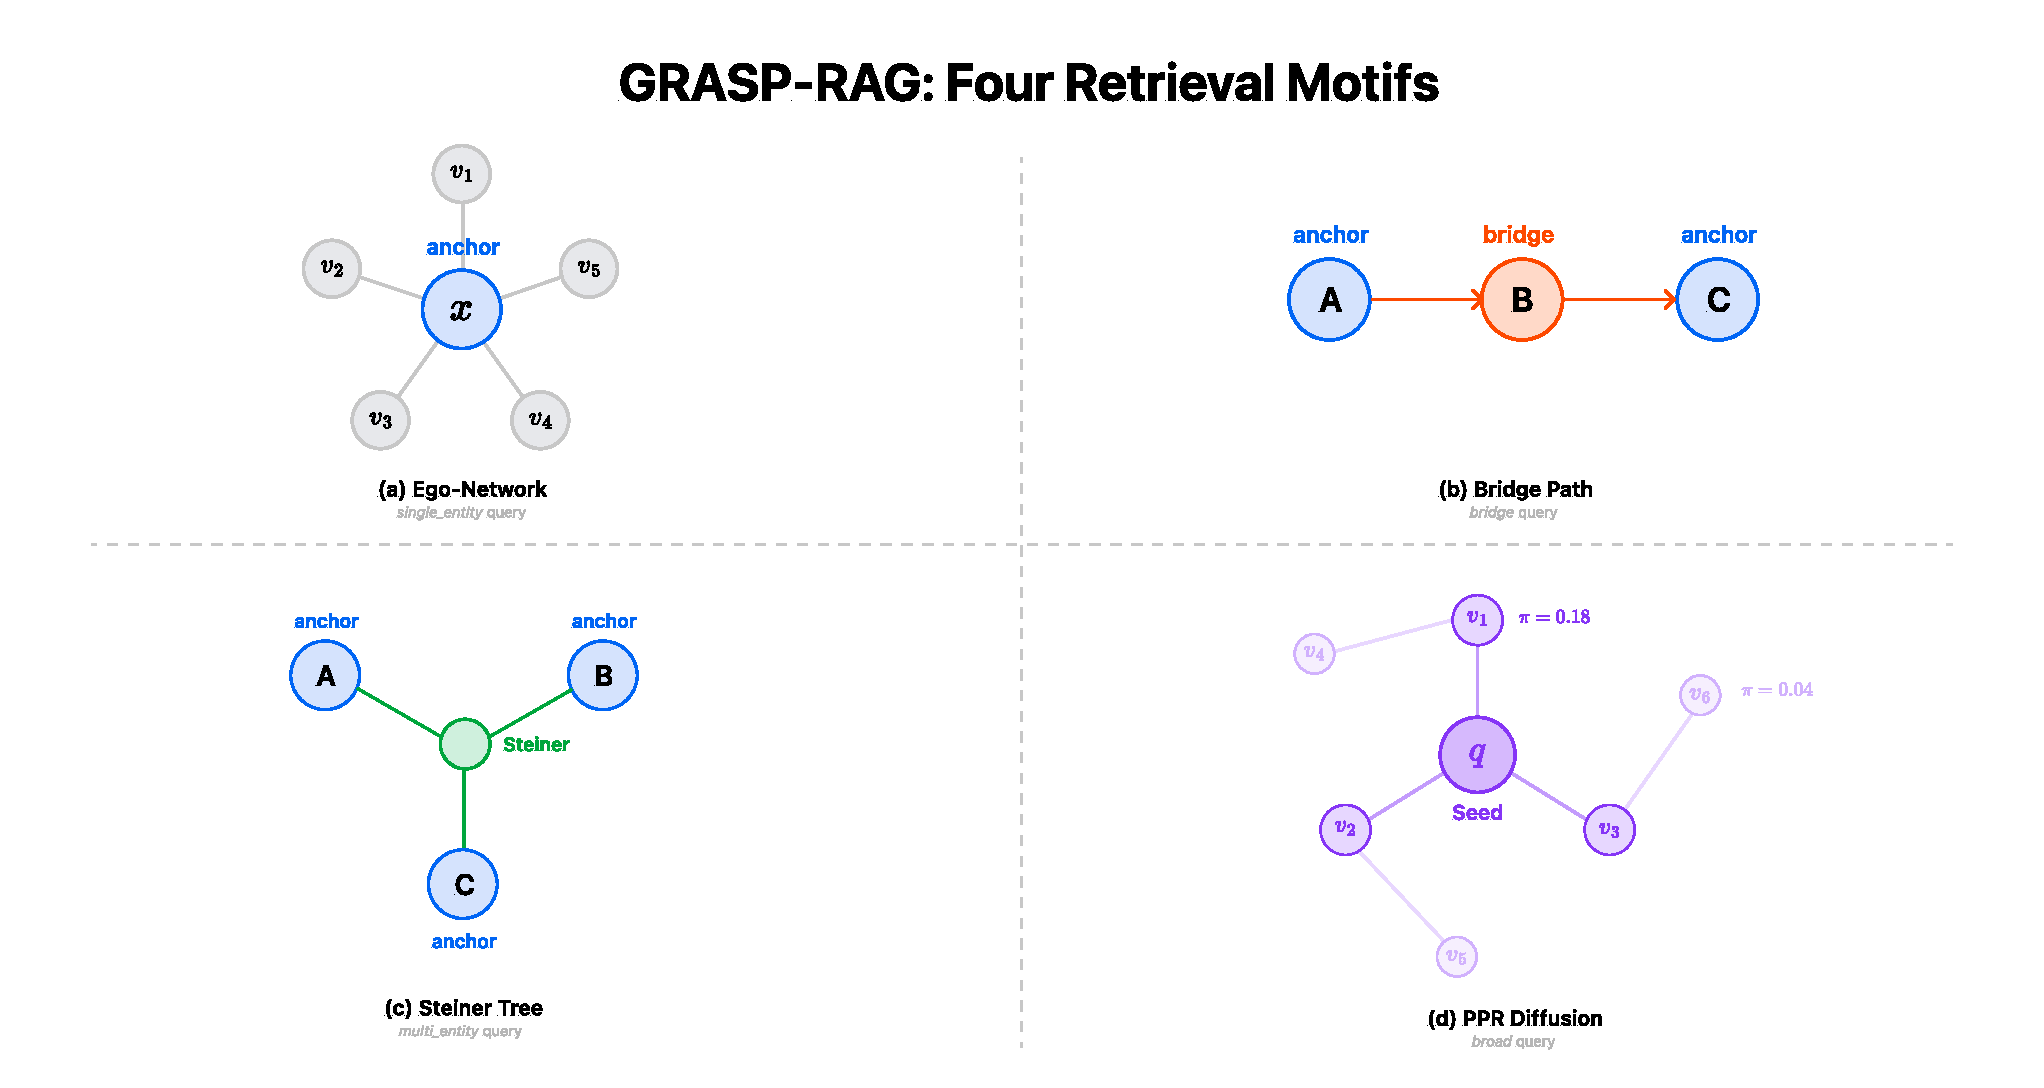
\includegraphics[width=\columnwidth]{fig_motifs.pdf}
  \caption{The four GRASP-RAG retrieval motifs. Blue nodes are query anchors;
    orange is the bridge intermediate entity; green is a Steiner intermediate
    node. Each motif targets the subgraph shape required by the corresponding
    query type; the broad motif delegates to LightRAG hybrid (not shown).}
  \label{fig:motifs}
\end{figure}
